\documentclass[12pt,a4paper]{article}

% Packages
\usepackage{geometry}
\geometry{margin=1in}
\usepackage{fancyhdr}
\usepackage{titlesec}
\usepackage{listings}
\usepackage{xcolor}
\usepackage{graphicx} 

% Header & Footer
\pagestyle{fancy}
\fancyhf{}
\rhead{OOP Java - Assignment 3}
\lhead{Kamithkar Vinod}
\cfoot{\thepage}

% Title formatting
\titleformat{\section}{\large\bfseries}{Problem \thesection:}{0.5em}{}
\titleformat{\subsection}[runin]{\bfseries}{Code:}{0.5em}{}[---]
\titleformat{\subsubsection}[runin]{\bfseries}{Output:}{0.5em}{}[---]

% Code style
\lstset{
    language=Java,
    basicstyle=\ttfamily\small,
    keywordstyle=\color{blue}\bfseries,
    commentstyle=\color{gray}\itshape,
    stringstyle=\color{red},
    showstringspaces=false,
    numbers=left,
    numberstyle=\tiny\color{gray},
    frame=single,
    breaklines=true
}

% Document Start
\begin{document}

% Title Page
\begin{center}
    \LARGE \textbf{Assignment - 3} \\[0.5cm]
    \Large \textbf{Object-Oriented Programming in Java} \\[1cm]

    \begin{tabular}{rl}
        \textbf{Name:} & Kamithkar Vinod \\
        \textbf{Course:} & PG DAC AUGUST 2025 \\
        \textbf{Form No:} & 250500480 \\
        \textbf{Date:} & 14-09-2025 \\
    \end{tabular}
\end{center}

\vspace{1cm}
\hrule
\vspace{0.5cm}

% Problems

\section{Grading System -- else if}
\textbf{Task:} Write a program that takes a student's percentage as input and assigns a grade based on the
following criteria:
\begin{itemize}
    \item 90\% and above $\rightarrow$ Grade A
    \item 80\% to 89\% $\rightarrow$ Grade B
    \item 70\% to 79\% $\rightarrow$ Grade C
    \item 60\% to 69\% $\rightarrow$ Grade D
    \item Below 60\% $\rightarrow$ Grade F
\end{itemize}

\subsection{}
\begin{lstlisting}
import java.util.Scanner;
class PercentageElseIf{
    public static void main(String[] args) {
        Scanner scanner = new Scanner(System.in);
        // taking percentage from the end user
        System.out.print("Enter your percentage: ");
    
        // check if input is numeric
        if (!scanner.hasNextDouble()){
            System.out.println("Invalid Input: Enter a number between 0 to 100");
            return;
        }
    
        double percentage = scanner.nextDouble();
    
        // validate percentage range
        if (percentage < 0 || percentage > 100) {
            System.out.println("Invalid Percentage! Please enter a value between 0 and 100");
            return;
        }
    
        int grade = (int) (percentage / 10);
    
        if (grade >= 9 && grade <= 10) 
            System.out.println("Grade: A");
        else if (grade >= 8 && grade < 9) 
            System.out.println("Grade: B");
        else if (grade >= 7 && grade < 8)
            System.out.println("Grade: C");
        else if (grade >= 6 && grade < 7)
            System.out.println("Grade: D");
        else
            System.out.println("Grdae: F");
    }
}
\end{lstlisting}

\subsubsection{}
\begin{center}
    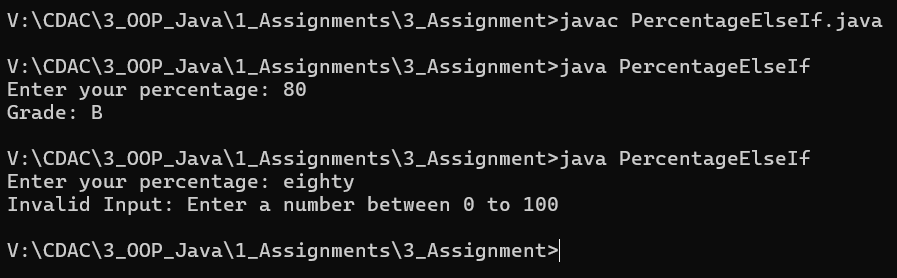
\includegraphics[width=0.8\textwidth]{1_percentage_else_if.png}
\end{center}

\section{Grading System -- switch case}
\textbf{Task:} Write a program that takes a student's percentage as input and assigns a grade based on the
following criteria:
\begin{itemize}
    \item 90\% and above $\rightarrow$ Grade A
    \item 80\% to 89\% $\rightarrow$ Grade B
    \item 70\% to 79\% $\rightarrow$ Grade C
    \item 60\% to 69\% $\rightarrow$ Grade D
    \item Below 60\% $\rightarrow$ Grade F
\end{itemize}

\subsection{}
\begin{lstlisting}
import java.util.Scanner;
class GradingSwitch {
    public static void main(String[] args) {
        Scanner scanner = new Scanner(System.in);
    
        System.out.print("Enter your percentage: ");
    
        // check if input is numeric
        if (!scanner.hasNextDouble()) {
            System.out.println("Invalid Input: Please enter the values between 0 to 100");
            return;
        }
    
        double percentage = scanner.nextDouble();
    
        // validate percentage range
        if (percentage < 0 || percentage > 100){
            System.out.println("Invalid Percentage");
            return;
        }
    
        int grade = (int) (percentage / 10);
    
        switch (grade){
        case 10:
        case 9: System.out.println("Grade: A"); break;
        case 8: System.out.println("Grade: B"); break;
        case 7: System.out.println("Grade: C"); break;
        case 6: System.out.println("Grade: D"); break;
        default:
            System.out.println("Grade: F");
            break;
        }
    }
}
\end{lstlisting}

\subsubsection{}
\begin{center}
    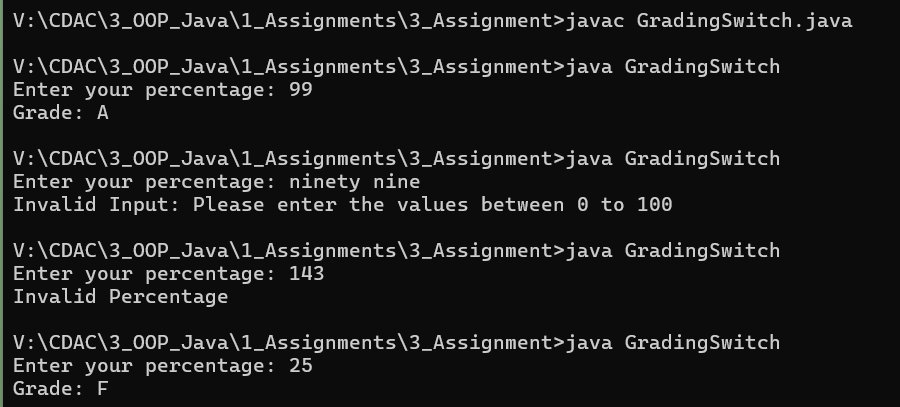
\includegraphics[width=0.8\textwidth]{2_percentage_else_if.png}
\end{center}

\section{Electricity Bill Calculation -- else if}
\textbf{Task:} Write a program that calculates the electricity bill based on the number of units consumed. The charges per unit are as follows:
\begin{enumerate}
    \item For the first 100 units: ₹5 per unit
    \item For 101--200 units: ₹6 per unit
    \item For 201--300 units: ₹7 per unit
    \item For above 300 units: ₹8 per unit
\end{enumerate}

\subsection{}
\begin{lstlisting}
import java.util.Scanner;
class ElectrcityBillCalculationElseIf {
    public static void main(String[] args) {
        Scanner scanner = new Scanner(System.in);
        System.out.print("Enter the Electricity consumed units: ");
        // check if input 
        if (!scanner.hasNextDouble()) {
            System.out.println("Invalid Input");
            return;
        }
    
        double units = scanner.nextDouble();
    
        // validate the range
        if (units <= 0){
            System.out.println("Please enter the units greater than 0");
            return;
        }
        
        double amount;
    
        if (units <= 100) {
            amount = units * 5;
        }
        else if (units > 100 && units <= 200) {
            amount = (100 * 5) + ((units - 100) * 6);
        }
        else if (units > 200 && units <= 300) {
            amount = (100 * 5) + (100 * 6) + ((units - 200) * 7); 
        }
        else {
            amount = (100 * 5) + (100 * 6) + (100 * 7) + ((units - 300) * 8);
        }
        System.out.println("Electricity Bill Amount: " + amount);
    }
}
\end{lstlisting}

\subsubsection{}
\begin{center}
    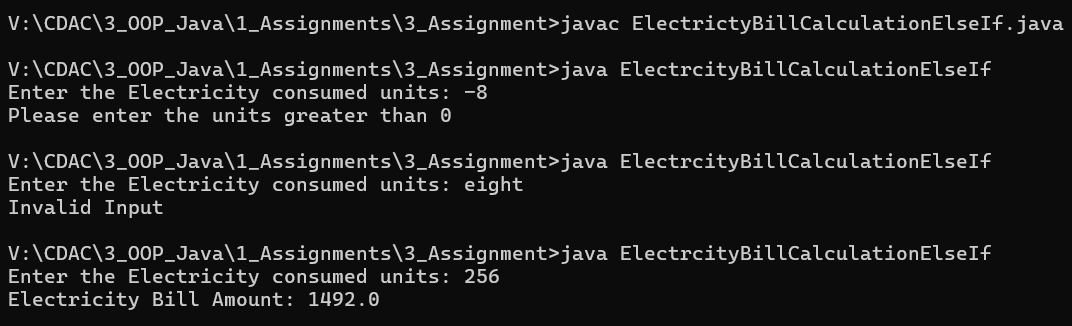
\includegraphics[width=0.8\textwidth]{3_electricity_else_if.png}
\end{center}

\section{Electricity Bill Calculation -- switch case}
\textbf{Task:} Write a program that calculates the electricity bill based on the number of units consumed. The charges per unit are as follows:
\begin{enumerate}
    \item For the first 100 units: ₹5 per unit
    \item For 101--200 units: ₹6 per unit
    \item For 201--300 units: ₹7 per unit
    \item For above 300 units: ₹8 per unit
\end{enumerate}

\subsection{}
\begin{lstlisting}
import java.util.Scanner;
class ElectrcityBillCalculationSwitch {
    public static void main(String[] args) {
        Scanner scanner = new Scanner(System.in);
        System.out.print("Enter the Electricity consumed units: ");
        // check if input 
        if (!scanner.hasNextDouble()) {
            System.out.println("Invalid Input");
            return;
        }
    
        double units = scanner.nextDouble();
    
        // validate the range
        if (units <= 0){
            System.out.println("Please enter the units greater than 0");
            return;
        }
        
        int u = (int) (units / 100);
    
        double amount;
    
        switch (u) {
        case 0: {
            amount = units * 5;
            break;
        }
        case 1: {
            amount = (100 * 5) + ((units - 100) * 6);
            break;
        }
        case 2: {
            amount = (100 * 5) + (100 * 6) + ((units - 200) * 7);
            break;
        }
        default: {
            amount = (100 * 5) + (100 * 6) + (100 * 7) + ((units - 300) * 8);
        }
        }
        System.out.println("Electricity Bill Amount: " + amount);
    }
}
\end{lstlisting}

\subsubsection{}
\begin{center}
    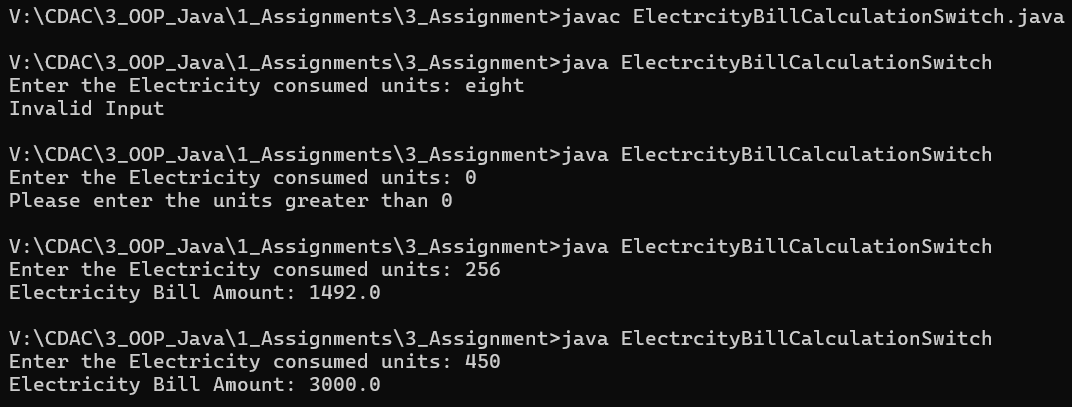
\includegraphics[width=0.8\textwidth]{4_electricity_switch.png}
\end{center}

\section{Income Tax Calculation -- else if }
\textbf{Task:} Write a program that calculates the income tax payable based on the annual salary:
\begin{enumerate}
    \item Income $\leq$ ₹2,50,000 : No tax
    \item ₹2,50,001 -- ₹5,00,000 : 5\% tax
    \item ₹5,00,001 -- ₹10,00,000 : 20\% tax
    \item Above ₹10,00,000 : 30\% tax
\end{enumerate}

\subsection{}
\begin{lstlisting}
import java.util.Scanner;
class IncomeTaxCalcElseIf {
    public static void main(String[] args) {
        Scanner scanner = new Scanner(System.in);
        System.out.print("Enter your Income: ");
    
        // check if input is numeric
        if (!scanner.hasNextDouble()){
            System.out.println("Invalid Input");
            return;
        }
    
        double income = scanner.nextDouble();
    
        // validate the range
        if (income <= 0) {
            System.out.println("Please enter Income greater than 0");
            return;
        }
        double tax;
    
        if (income <= 250000) {
            tax = 0;
        }
        else if (income > 250000 && income <= 500000) {
            tax = (income - 250000) * (5.0/100);
        }
        else if (income > 500000 && income <= 1000000) {
            tax = (250000 * (5.0/100)) + ((income - 500000) * (20.0/100)) ;
        }
        else {
            tax = (250000 * (5.0/100)) + (500000 * (20.0/100)) + ((income - 1000000) * (30.0/100));
        }
        System.out.println("The tax for income " + income + " is : " + tax);
    }
}
\end{lstlisting}

\subsubsection{}
\begin{center}
    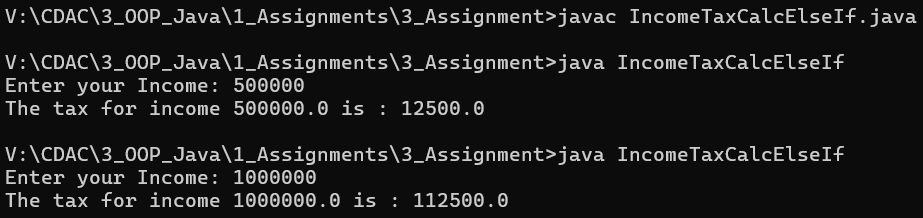
\includegraphics[width=0.8\textwidth]{5_incometax_elseif.png}
\end{center}

\section{Income Tax Calculation -- switch case }
\textbf{Task:} Write a program that calculates the income tax payable based on the annual salary:
\begin{enumerate}
    \item Income $\leq$ ₹2,50,000 : No tax
    \item ₹2,50,001 -- ₹5,00,000 : 5\% tax
    \item ₹5,00,001 -- ₹10,00,000 : 20\% tax
    \item Above ₹10,00,000 : 30\% tax
\end{enumerate}

\subsection{}
\begin{lstlisting}
import java.util.Scanner;
class IncomeTaxCalcSwitch {
    public static void main(String[] args) {
        Scanner scanner = new Scanner(System.in);
        System.out.print("Enter your Income: ");
    
        // check if input is numeric
        if (!scanner.hasNextDouble()){
            System.out.println("Invalid Input");
            return;
        }
    
        double income = scanner.nextDouble();
    
        // validate the range
        if (income <= 0) {
            System.out.println("Please enter Income greater than 0");
            return;
        }
        double tax = 0.0;
    
        int slab;
    
        // decide slab index
        if (income <= 250000) {
            slab = 0;
        }
        else if (income <= 500000){
            slab = 1;
        }
        else if (income <= 1000000){
            slab = 2;
        }
        else {
            slab = 3;
        }
    
        switch (slab) {
        case 0: // upto 2.5L
            tax = 0; break;
        case 1: // upto 5L
            tax = (income - 250000) * (5.0/100); break;
        case 2: // upto 10L
            tax = (250000 * (5.0/100)) + ((income - 500000) * (20.0/100)) ;
            break;
        case 3: // above 10l
            tax = (250000 * (5.0/100)) + (500000 * (20.0/100)) + ((income - 1000000) * (30.0/100));
            break;
        default:
            System.out.println("Error in Calculating Tax");
        }
        System.out.println("The tax for income " + income + " is : " + tax);
    }
}
\end{lstlisting}

\subsubsection{}
\begin{center}
    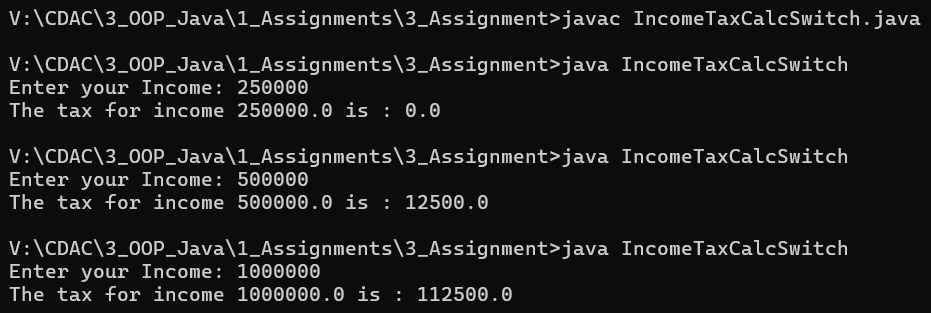
\includegraphics[width=0.8\textwidth]{6_incometax_switch.png}
\end{center}



\end{document}
